
\documentclass[12pt]{article}

\usepackage[T1]{fontenc}
\usepackage{float}
\usepackage[utf8]{inputenc}
\usepackage[french]{babel}
\usepackage{hyperref}
\usepackage{amsmath}
\usepackage{amssymb}
\usepackage[top=1.5cm, bottom=1.5cm, left=1.5cm, right=1.5cm]{geometry}
\usepackage{graphicx}
\usepackage{multicol}
\usepackage{lipsum}
\usepackage{eurosym}
\usepackage{indentfirst}
\usepackage{titlesec}
\usepackage{pifont}
\usepackage{url}
\usepackage{epsf}
\usepackage{listings}
\newcommand\tab[1][1cm]{\hspace*{#1}}
\begin{document}
    \begin{titlepage}
        \newcommand{\HRule}{\rule{\linewidth}{0.5mm}}
        \center
        \textsc{\LARGE
        UNIVERSITE CAEN-NORMANDIE
        } \\[1cm]
        
\includegraphics[scale=1]{images/LOGO-UNICAEN_V-2.2-N} \\[1cm]
        \HRule \\[0.4cm]
        { \huge \bfseries Rapport de développement: EasyTasK\\[0.15cm] }
        \HRule \\[1.5cm]
        KITSOUKOU Manne Emile\\[1cm]
        ALSEINY
        \\[1cm]
        \textbf{Licence 3 Informatique}\\
        \today \\ [1cm]
    \end{titlepage}
    \newpage
    \tableofcontents
    \newpage
    \section{Introduction}\label{sec:intro}

        Dans le cadre de la validation de l'UE( Unité d'Enseignement) de \textbf{Développement d'application web client},
        nous avons été amenés à réaliser une application de gestions de tâches. L'objectif de ce projet était de mettre
        en place une interface utilisateur intuitive, fonctionnel et ergonomique permettant à un utilisateur de gérer
        ses listes de tâches de manière simple, intuitive et efficace.\\

        Ce projet nous a permis de découvrir le framework \textbf{React native } tout en mettant en pratique nos
        connaissances en développement d'application mobiles. Nous avons dû faire face à des défis liés à la prise
        en main de ce nouvel outil, mais avons réussi à mettre en place une application fonctionnelle et ergonomique
        respectant les exigences de l'énoncé du projet. Cela a été également l'occassion de mettre en pratique nos
        connaissances des bases de données non traditionnelles à travers la mise en place d'une base de données
        \textbf{NoSQL} \textbf{GRAPHQL} à travers le service \textbf{Apollo NEO4J}.

        \section{Fonctionnalités}\label{sec:fonctionnalites}

        EasyTask offre à l'utilisateur une panoplie de fonctionnalités lui permettant de gérer ses différentes tâches.
        Ces fonctionnalités sont divisées en deux grandes catégories : les fonctionnalités de base et les fonctionnalités
        avancées.
        En parlant de fonctionnalités de base, nous faisons référence aux fonctionnalités non seulement classiques
        et indispensables à une application de gestion de tâches, mais aussi à celles qui ne nécessitent pas de grande
        complexité de développement.
        Les fonctionnalités avancées quant à elles, font allusion à des fonctionnalités
        dont le développement est beaucoup moins intuitif et qui nécessitent une bonne connaissance des outils utilisés
        pour leur mise en place.\\

        \subsection{Fonctionnalités de base}\label{subsec:fonctionnalites-de-base}
        Ces fonctionnalités constituent les fondations de l'application. Elles ont été conçues pour répondre aux
        besoins qu'un utilisateur lambda peut avoir en matière de gestion de tâches. C'est à dire, ce sont des fonctionnalités
        qui aideront l'utilisateur à gérer ses tâches de manière simple et intuitive.\\

        \subsubsection{Authentification}\label{subsubsec:authentification}
        L'authentification est la première fonctionnalité que l'utilisateur doit utiliser pour pouvoir utiliser l'application.
        Elle permet à l'utilisateur de se connecter à son compte et d'accéder à ses tâches.
        En effet, l'application a été développée avec la volonté de ne pas stocker les données de l'utilisateur en local sur son appareil.
        De ce fait, il a fallu associer les tâches de l'utilisateur à son compte pour pouvoir les récupérer à chaque
        fois connexion et ne pas les perdre ni créer des conflits entre les données de plusieurs utilisateurs.\\

        % Afficher les 2 écrans de connexion et d'inscription cote à cote sur la même ligne
        \begin{figure}[H]
            \centering
            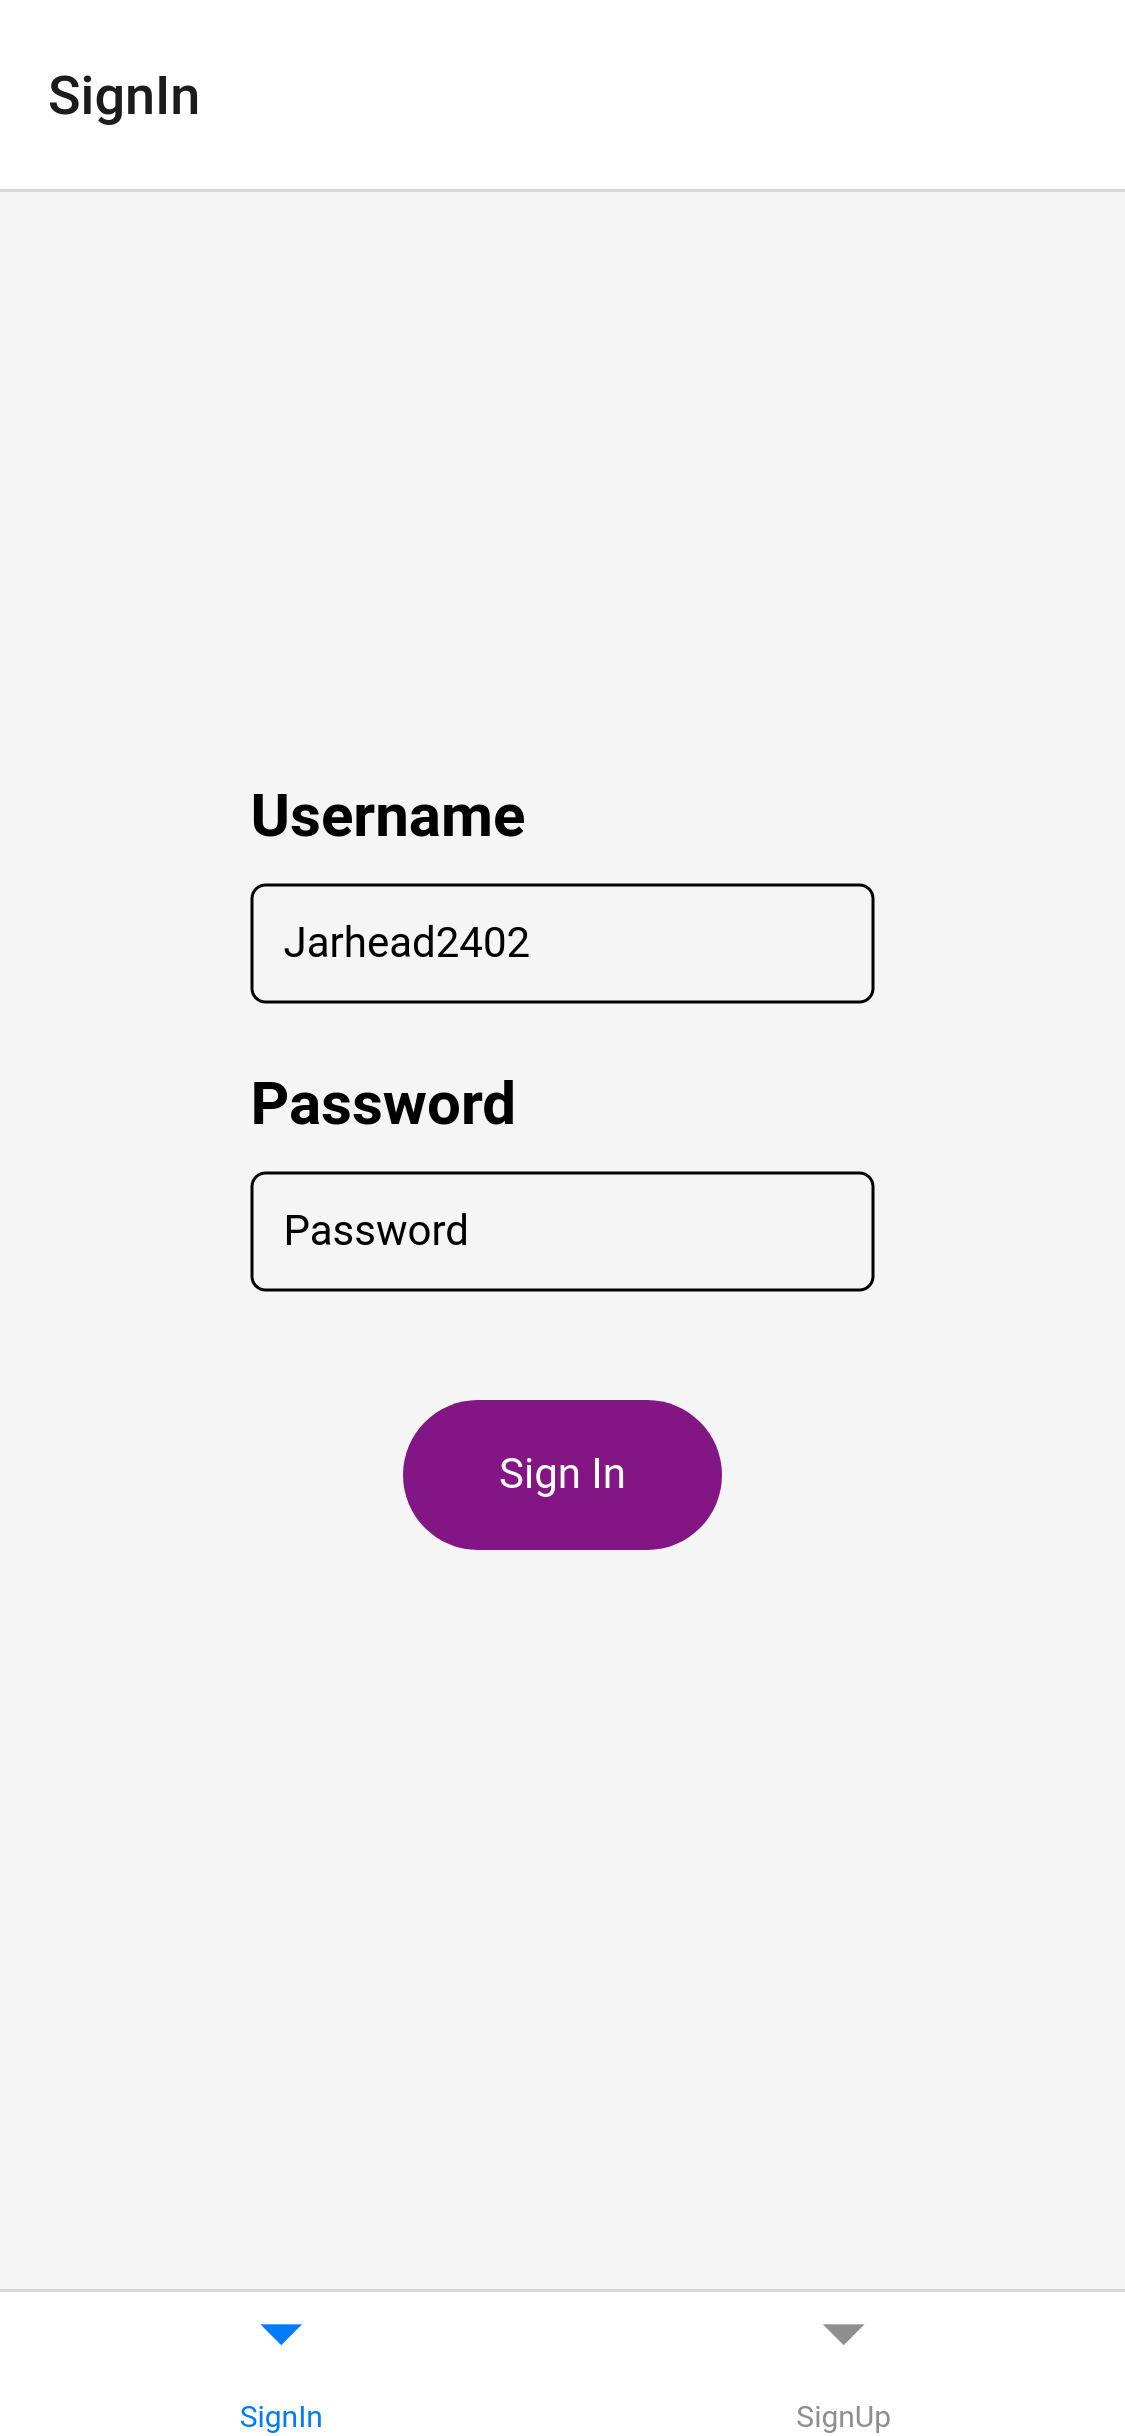
\includegraphics[width=0.45\textwidth]{images/signIn}
            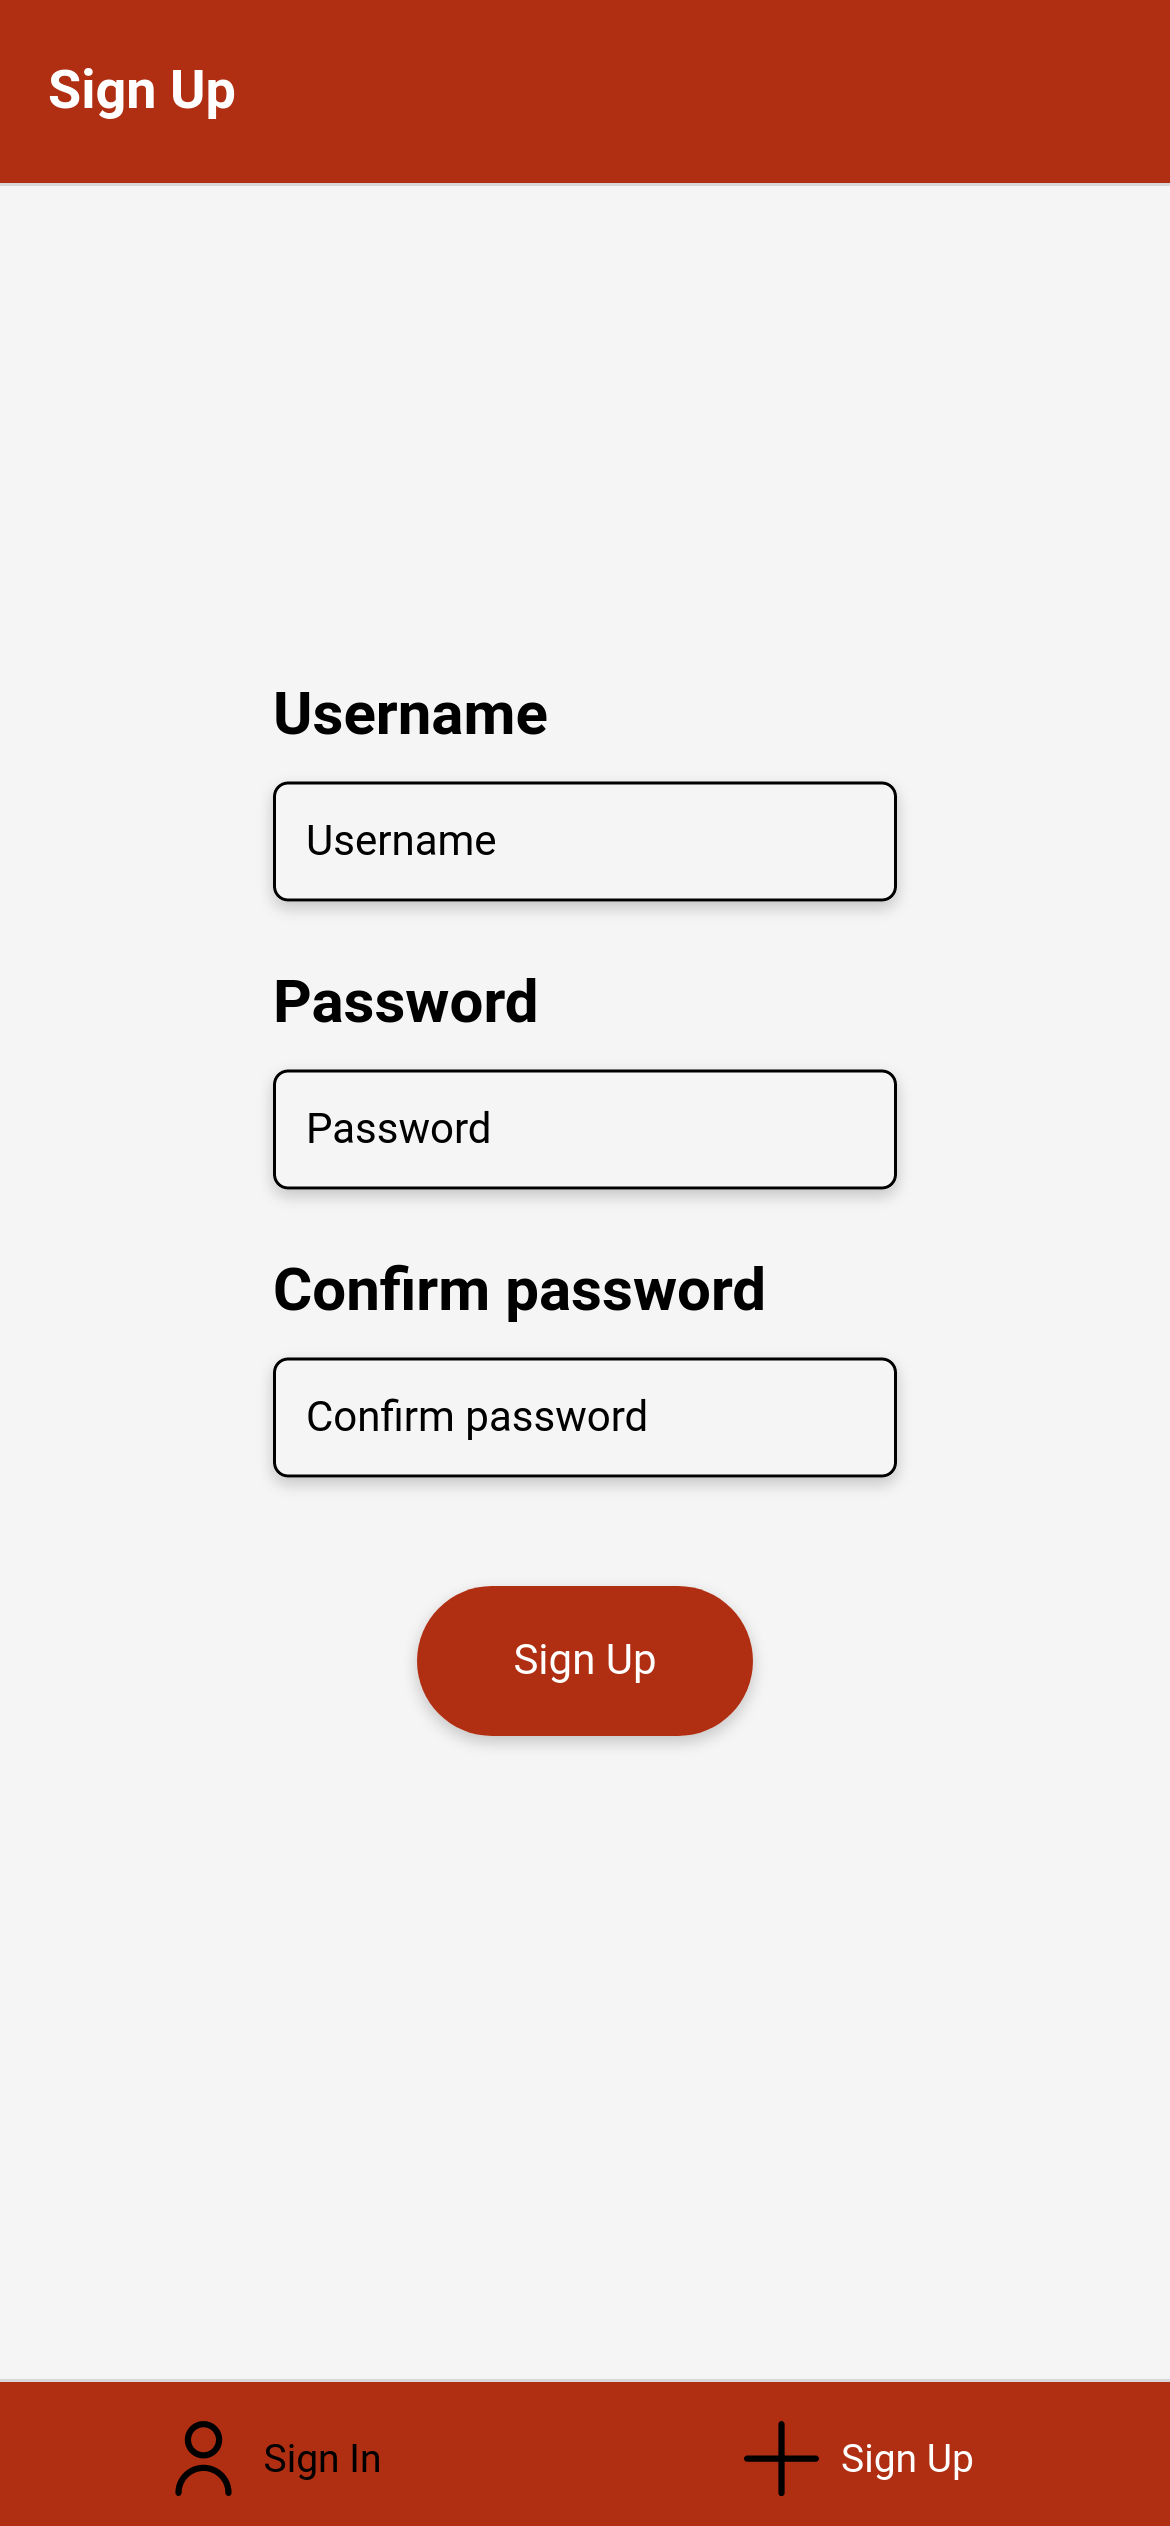
\includegraphics[width=0.45\textwidth]{images/signUp}
            \caption{Ecran de connexion et d'inscription}
            \label{fig:connexion}
        \end{figure}

        Un utilisateur qui souhaite utiliser l'application doit donc se créer un compte en renseignant son nom d'utilisateur,
        et son mot de passe\footnote{Le mot de passe doit être robuste, c'est à dire qu'il doit contenir au moins 8 caractères, dont au moins
        une lettre majuscule, une lettre minuscule, un chiffre. Cela permet de garantir la sécurité du compte de l'utilisateur
        dans le cas où celui-ci est piraté. De plus il faudrait dans une version ultérieure de l'application, hasher le mot de passe de l'utilisateur avant
        de le stocker dans la base de données}
        Une fois le compte créé, l'utilisateur peut se connecter à son compte en renseignant ces mêmes
        informations et accéder à ses tâches.\\

        \subsubsection{Manipulation des tâches}\label{subsubsec:manipulation-des-taches}
        Une fois connecté à son compte, l'utilisateur peut accéder à ses tâches. Il peut alors créer une nouvelle tâche,
        modifier le statut d'une tâche, ou encore supprimer une tâche. Dans la version actuelle de l'application, le statut
        d'une tâche se limite à : \textbf{todo}\footnote{La tâche n'a pas encore été effectuée}, \textbf{done}\footnote{La tâche a été effectuée}.

        % Afficher l'écran de gestion des tâches
        \begin{figure}[H]
            \centering
            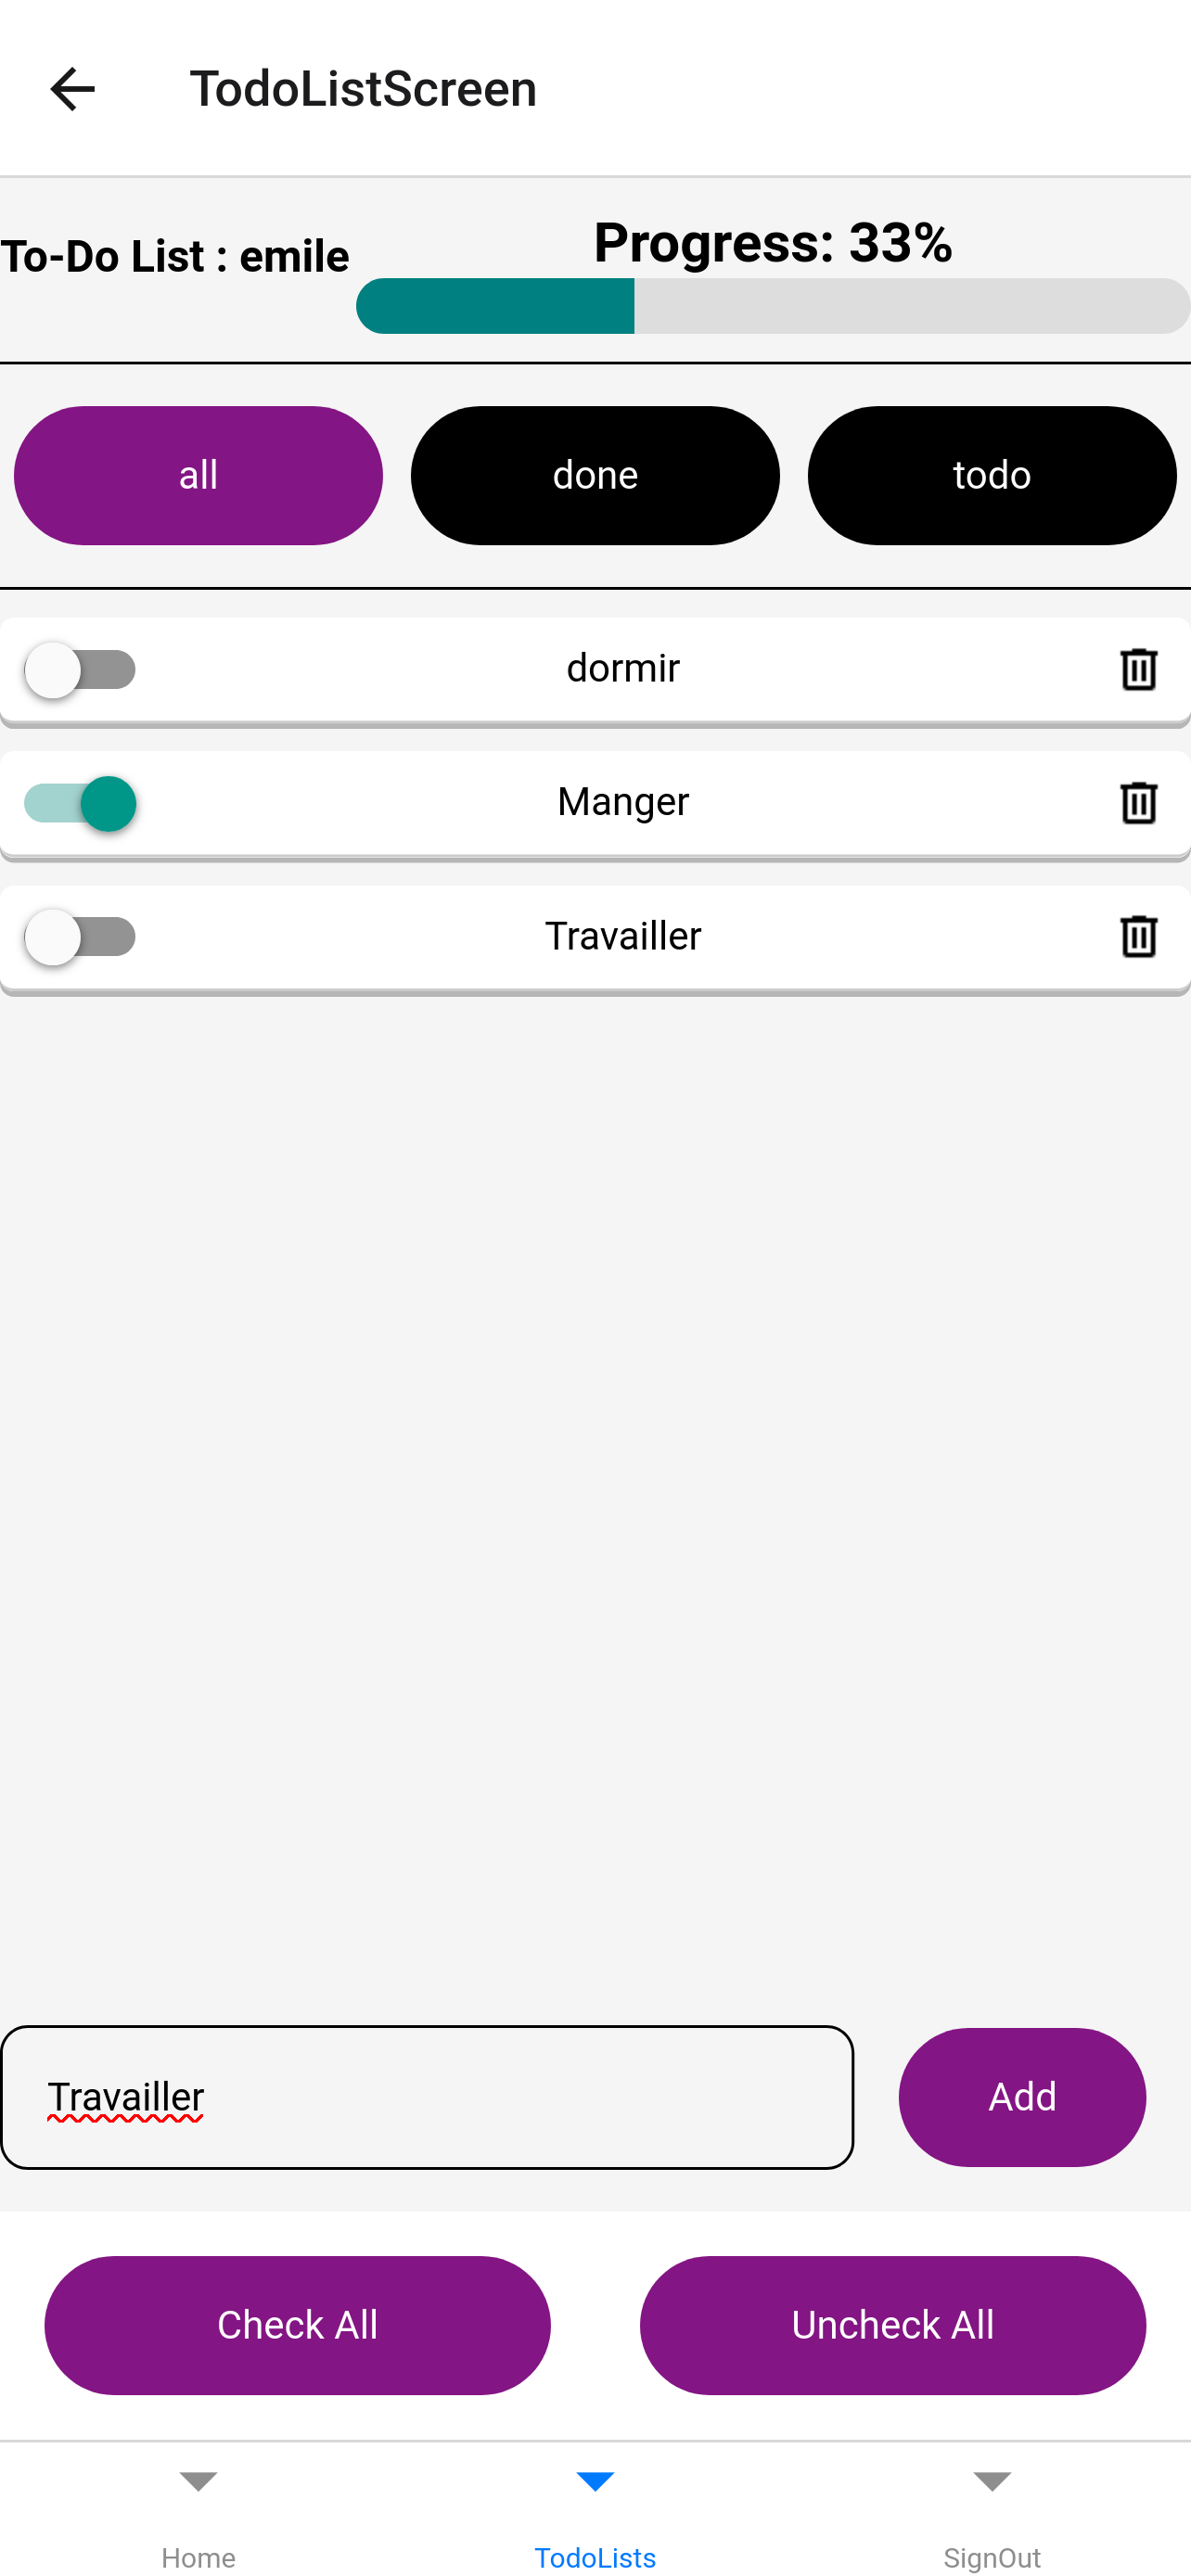
\includegraphics[width=0.45\textwidth]{images/tasks}
            \caption{Ecran de gestion des tâches}
            \label{fig:gestion-taches}
        \end{figure}

        Comme on peut le voir sur la figure \ref{fig:gestion-taches}, l'utilisateur peut créer une nouvelle tâche en
        remplissant le champ de texte en dessous de l'écran et en cliquant sur le bouton \textbf{Add}. Le choix
        a été fait de ne pas laisser la possibilité à l'utilisateur de créer une tâche vide. Cela permet de garantir
        que l'utilisateur ne crée pas de tâche sans contenu qui sont souvent inutiles et qui pollueront la liste des tâches.\\
        Le changement de statut d'une tâche se fait en cliquant sur le bouton \textbf{switch} à côté de la tâche et la suppression
        d'une tâche se fait en cliquant sur l'icône \textbf{trash} à côté de la tâche\footnote{La suppression d'une tâche est définitive et sans possibilité de récupération}\\

        Toutefois, il faut noter que l'utilisateur peut filtrer les tâches en fonction de leur statut. Il peut ainsi
        afficher uniquement les tâches qui sont à faire ou celles qui ont déjà été effectuées et donc mieux gérer ses tâches.\\
        Une possibilité lui a été aussi donnée de rendre toutes ses tâches à faire en cliquant sur le bouton \textbf{Reset} ou
        de les marquer toutes comme effectuées en cliquant sur le bouton \textbf{Done}.\\

        \subsection[Bonus]{Fonctionnalités avancées}\label{subsec:fonctionnalites-avancees}
        Ces fonctionnalités sont des fonctionnalités qui ont été ajoutées à l'application pour améliorer l'expérience utilisateur.
        Certaines d'entre elles sont uniquement des questions de confort, style ou de design, d'autres par contre sont
        des fonctionnalités qui permettent d'augmenter la productivité de l'utilisateur et emmènent l'application vers
        une autre dimension d'utilisation.\\

        \subsubsection{Gestions des listes de tâches}\label{subsubsec:gestion-des-listes-de-taches}
        Dans une application de gestion de tâches, on peut se retrouver avec une liste de tâches très longue et
        très difficile à gérer. De plus, il peut être intéressant de pouvoir regrouper des tâches en fonction de leur
        thème ou de leur catégorie.\\
        C'est pourquoi, EasyTasks permet à l'utilisateur de créer des listes de tâches. Il peut ainsi créer une liste
        de tâches pour ses tâches professionnelles, une autre pour ses tâches personnelles, une autre pour ses tâches
        de sport, etc.\\
        Cette fonctionnalité est un gros gain de productivité pour l'utilisateur, car il peut ainsi mieux organiser ses tâches
        à sa convenance.

        % Afficher l'écran de gestion des listes de tâches
        \begin{figure}[H]
            \centering
            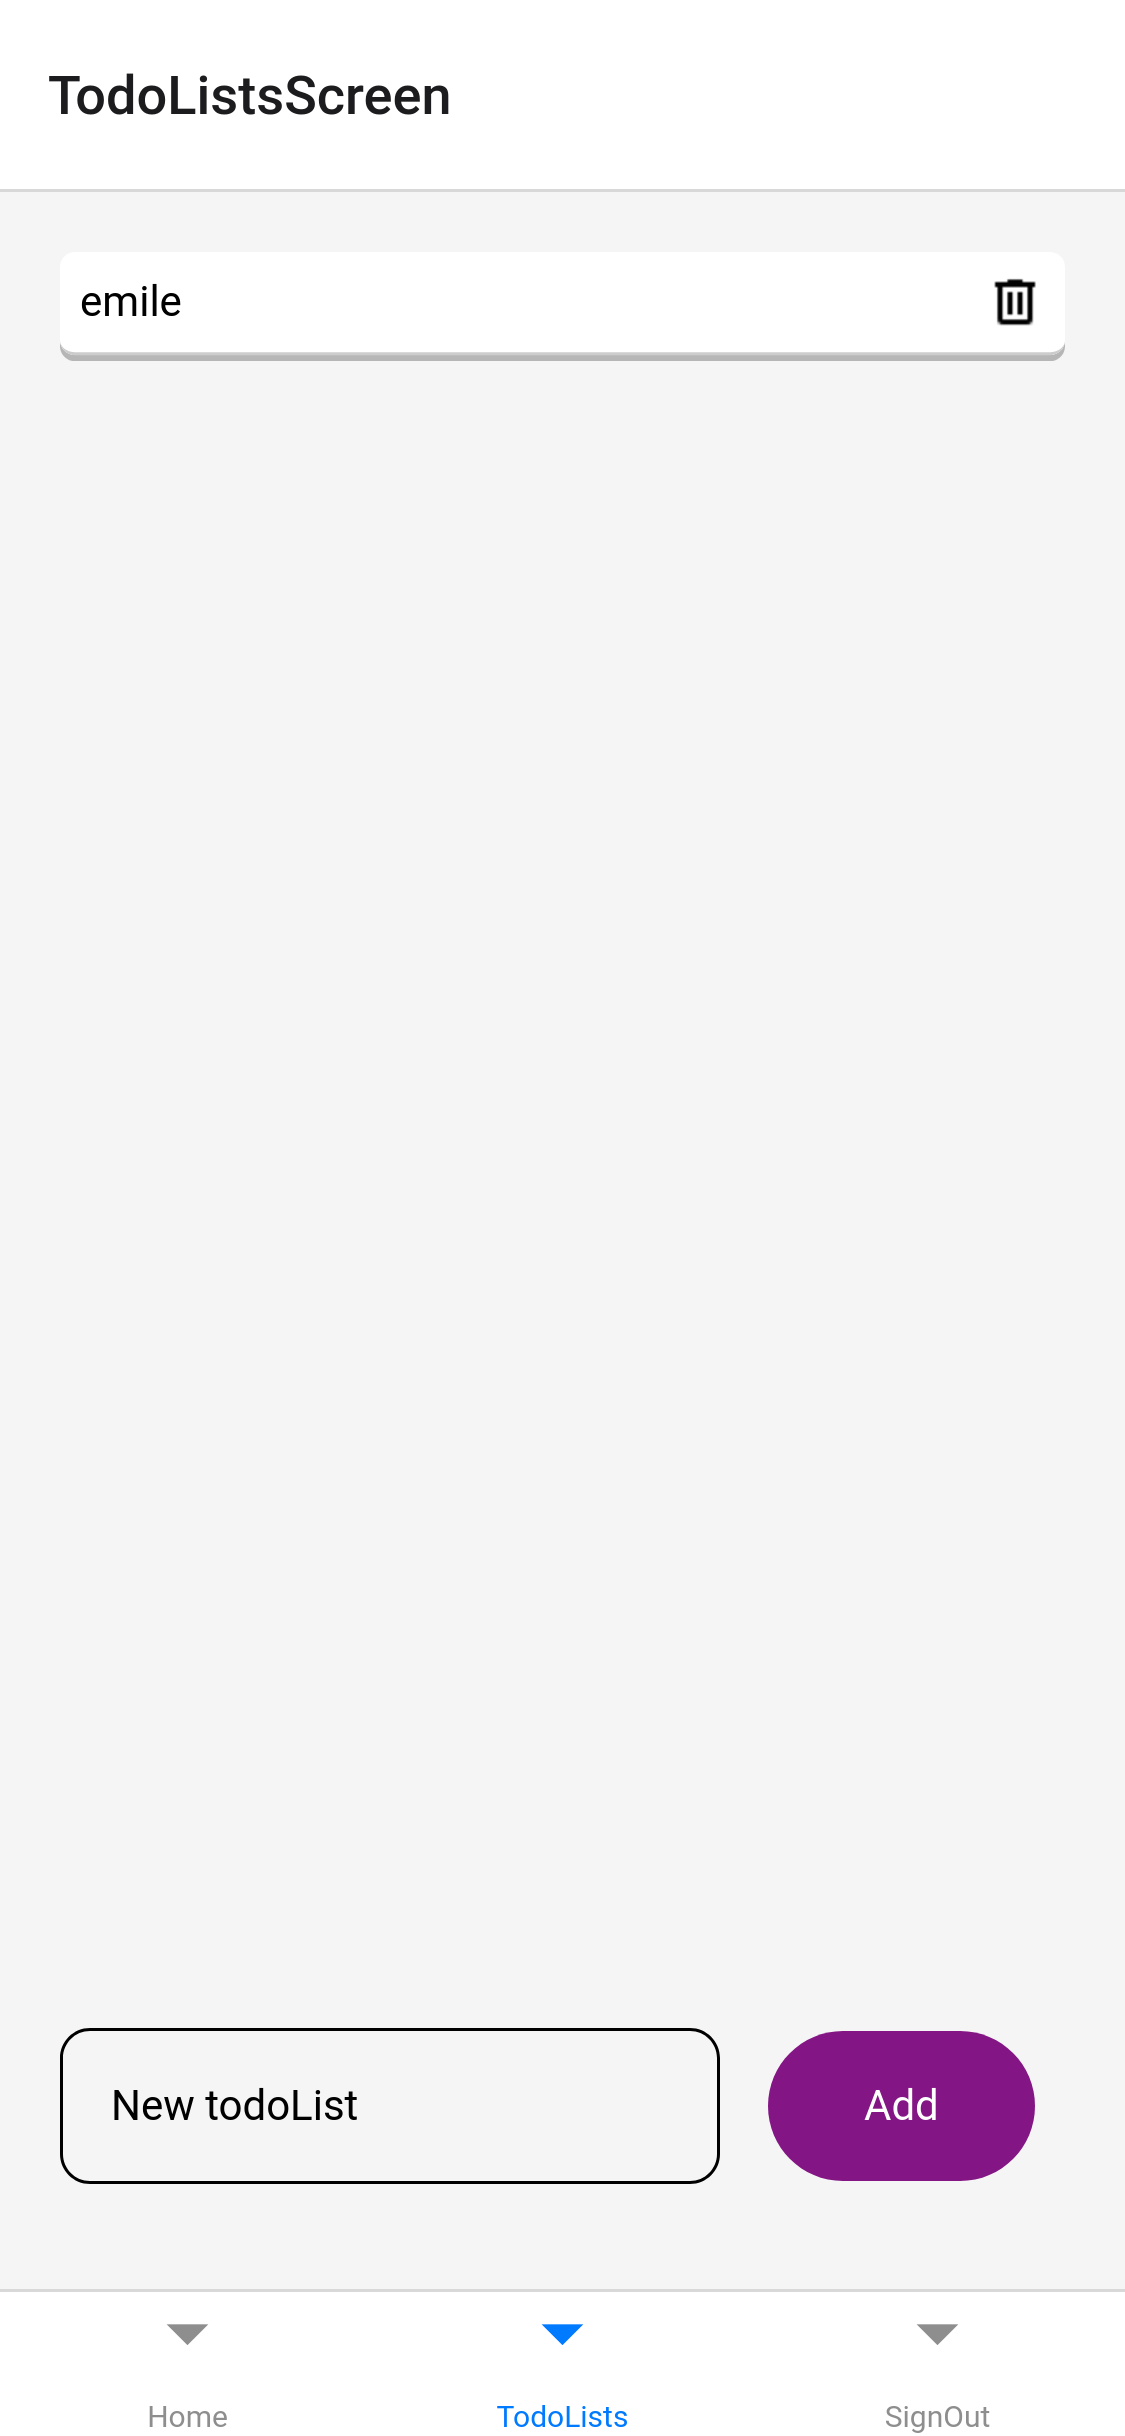
\includegraphics[width=0.45\textwidth]{images/taskList}
            \caption{Ecran de gestion des listes de tâches}
            \label{fig:gestion-listes}
        \end{figure}

        L'utilisateur peut créer une nouvelle liste de tâches voir la figure \ref{fig:gestion-listes} en remplissant
        le champ de texte et en cliquant sur le bouton \textbf{Add}.\\ Chaque item de la liste représente une liste de tâches
        et est cliquable. En cliquant sur un item, l'utilisateur est redirigé vers l'écran de gestion des tâches(voir figure \ref{fig:gestion-taches})
        et peut alors gérer les tâches de cette liste.\\
        La possibilité a été donnée à l'utilisateur de supprimer une liste de tâches en cliquant sur l'icône \textbf{trash}.
        Mais aussi de renommer une liste de tâches en maintenant pendant quelques secondes l'item de la liste.

        \section{Détails techniques}\label{sec:details-techniques}

        \section{Conclusion}\label{sec:conclusion}

        \section{Bibliographie}\label{sec:bibliographie}

        \bibliographystyle{plain}









\end{document}